\documentclass[../TDON2_inter.tex]{subfiles}%

\begin{document}
\section[s]"3"{Interférences ultrasonores sur un cercle}

\enonce{%
	\noindent
	\begin{minipage}{0.80\linewidth}
		Deux émetteurs E$_1$ et E$_2$ émettent des ondes ultrasonores de même
		fréquence $f = \SI{40}{kHz}$ (ce qui correspond à une longueur d'onde
		$\lambda = \SI{8.5}{nm}$) et en phase. On note O le milieu du segment [E$_1$
				E$_2$] de longueur $a = \SI{4}{cm}$, et (O$x$) l'axe situé sur la médiatrice
		de ce segment. On déplace le microphone sur un grand cercle de rayon $R =
			\SI{0.5}{m}$ et on relève l'évolution de l'amplitude mesurée en
		fonction de l'angle $\theta$ que fait la direction $\vec{\rm OM}$ avec l'axe
		(O$x$).
	\end{minipage}
	\hfill
	\begin{minipage}{0.20\linewidth}
		\begin{center}
			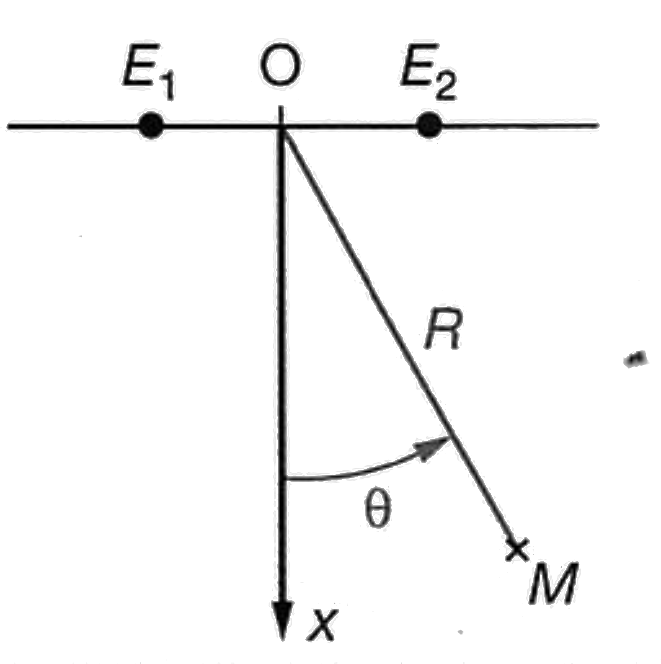
\includegraphics[width=\linewidth]{cercle-plain_white}
		\end{center}
	\end{minipage}
}

\begin{blocQR}
	\item
	\QR{%
		Faire une figure faisant apparaître les points O, E$_1$, E$_2$
		et M, pour un petit angle $\theta$ non nul.
	}{%
		On a
		\begin{center}
			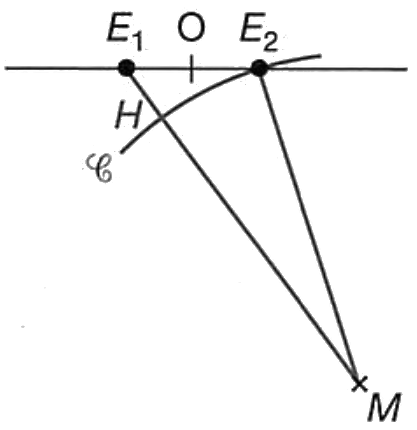
\includegraphics[width=0.2\linewidth]{cercle_corr-white}
		\end{center}
	}

	\QR{%
		Tracer l'arc de cercle de centre M passant par E$_2$. On note
		H son intersection avec la droite (E$_1$M). Que représente
		E$_1$H~?
	}{%
		E$_1$H est la différence ${\rm E_1M - E_2M} = r_1-r_2 = \D
			L_{1/2}(\Mr)$ avec les notations du cours~; autrement dit, c'est
		\fbox{la différence de marche} entre les deux ondes.
	}

	\QR{%
		Puisque $R \gg a$, on peut assimiler H et le projeté
		orthogonal de E$_2$ sur (E$_1$M). En déduire une expression du
		déphasage entre les ondes reçues en M en fonction de $\theta$,
		$a$ et $\lambda$.
	}{%
		En raisonnant dans le triangle $\rm E_1E_2H$, considéré rectangle, on
		a ${\rm E_1H} = a \sin\theta$. D'où le déphasage~:
		\[\boxed{\D\f_{2/1}(\Mr) = \frac{2\pi a\sin\theta}{\lambda}}\]
	}

	\QR{%
		Quelles sont, dans l'intervalle \SIrange{-30}{30}{\degree},
		les valeurs de $\theta$ où on observe un maximum d'amplitude~?
	}{%
		L'amplitude est maximale pour des interférences constructives, soit
		pour $\D\f_{2/1}(\Mr) = 2p\pi$ avec $p\in\Zb$~; sur $\theta$ ça donne
		donc
		\[
			\boxed{\sin\theta = p \frac{\lambda}{a}}
			\Lra
			\theta = \asin(p \frac{\lambda}{a})
		\]
		On regarde donc quels sont les ordres d'interférences $p$ tels que
		$\theta \in \SIrange{-30}{30}{\degree}$~:
		\begin{itemize}
			\item $p=0 \Rightarrow \theta = \ang{0;;}$, soit un maximum
			      pour tout l'axe $x$~: c'était attendu étant donné les symétries
			      du problème~;
			\item $p = \pm 1 \Rightarrow \theta = \pm\ang{12;;}$, donnant deux
			      points symétriques par rapport à (O$x$)~;
			\item $p = \pm 2 \Rightarrow \theta = \pm\ang{25;;}$, pratiquement
			      le double des valeurs précédentes.
		\end{itemize}
		$p > 2$ donne des valeurs en-dehors de l'intervalle.
	}

	\item
	\resetQ
	\QR{%
		Sur l'intervalle précédent, quelles sont les positions où un
		minimum d'amplitude est attendu~?
	}{%
		On a interférences destructives si $\D\f_{2/1}(\Mr) =
			(2p+1)\pi$, soit
		\[
			\boxed{\sin\theta = \left(p+\frac{1}{2}\right) \frac{\lambda}{a}}
			\Lra
			\theta = \asin(\left(p+\frac{1}{2}\right) \frac{\lambda}{a})
		\]
		\begin{itemize}
			\item $p=0 \Rightarrow \theta = \pm\ang{6;;}$~;
			\item $p=1 \Rightarrow \theta = \pm\ang{19;;}$.
		\end{itemize}
	}

	\QR{%
		Si les ondes émises ont même amplitude, quelle est la valeur
		minimale d'amplitude pour le signal somme~?
	}{%
		Pour des ondes reçues avec la même amplitude, l'opposition de
		phase conduit à une annulation totale de l'amplitude somme.
	}

\end{blocQR}

\end{document}
